\subsection{Algoritmi na grafih}

\begin{naloga}{?}{Vaje OR 20.4.2016}
\begin{vprasanje}[nal:matgraf]
Zasnuj podatkovno strukturo za grafe,
ki temelji na matrični predstavitvi.
Podatkovna struktura naj ima sledeče metode:
\begin{itemize}
\item {\tt \_\_init\_\_(G)}: ustvarjanje praznega grafa
\item {\tt dodajVozlisce(G, u)}: dodajanje novega vozlišča
\item {\tt dodajPovezavo(G, u, v)}: dodajanje nove povezave
\item {\tt brisiPovezavo(G, u, v)}: brisanje povezave
\item {\tt brisiVozlisce(G, u)}: brisanje vozlišča
\item {\tt sosedi(G, u)}: seznam sosedov danega vozlišča
\end{itemize}
Za vsako od naštetih metod podaj tudi njeno časovno zahtevnost
v odvisnosti od števila vozlišč, števila povezav in stopenj vhodnih vozlišč.
Oceni tudi prostorsko zahtevnost celotne strukture.
\end{vprasanje}
\begin{odgovor}
\end{odgovor}
\end{naloga}


\begin{naloga}{?}{Vaje OR 20.4.2016}
\begin{vprasanje}[nal:sosgraf]
Zasnuj podatkovno strukturo za grafe,
ki temelji na seznamih sosedov.
Zapiši metode kot pri prejšnji strukturi
ter oceni njihovo časovno zahtevnost
in prostorsko zahtevnost celotne strukture.
\end{vprasanje}
\begin{odgovor}
\end{odgovor}
\end{naloga}


\begin{naloga}{?}{Vaje OR 20.4.2016}
\begin{vprasanje}
Kako moramo spremeniti strukturi
iz nalog~\ref{nal:matgraf} in~\ref{nal:sosgraf},
da bosta predstavljali digrafe?
\end{vprasanje}
\begin{odgovor}
\end{odgovor}
\end{naloga}


\begin{naloga}{?}{Vaje OR 20.4.2016}
\begin{vprasanje}
Napiši algoritem, ki za vhodni graf $G$ določi, ali ima trikotnik.
Katero podatkovno strukturo za grafe boš uporabil?
\end{vprasanje}
\begin{odgovor}
\end{odgovor}
\end{naloga}


\begin{naloga}{?}{Vaje OR 4.5.2016}
\begin{vprasanje}
Dan je digraf $D = (V, E)$.
Pravimo, da je vozlišče $v \in V$ {\em zvezda} digrafa $D$,
če ima izhodno povezavo do vseh ostalih vozlišč
in v digrafu $D$ ni drugih povezav.
Napiši algoritem, ki poišče zvezdo danega digrafa, če ta obstaja.
\end{vprasanje}
\begin{odgovor}
\end{odgovor}
\end{naloga}


\begin{naloga}{Janoš Vidali}{Vaje OR 30.11.2016}
\begin{vprasanje}[nal:bfs]
Na grafu s slike~\ref{fig:bdfs} izvedi iskanje v širino.
V primerih, ko imaš več ena\-ko\-vred\-nih izbir,
upoštevaj abecedni vrstni red.
Za vsako povezavo določi, ali se nahaja v drevesu iskanja v širino.

\begin{figure}[t]
\centering
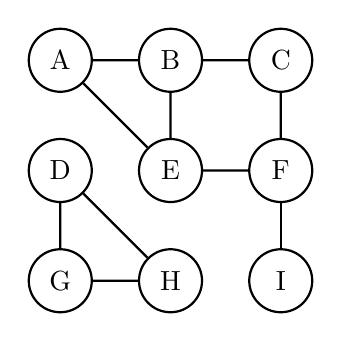
\begin{tikzpicture}[style=thick,scale=0.7]
\tikzstyle{vertex}=[draw, circle, fill=white, inner sep=0pt, minimum size=8mm]

\node[vertex] (A) at (-2, 2) {A};
\node[vertex] (B) at ( 0, 2) {B};
\node[vertex] (C) at ( 2, 2) {C};
\node[vertex] (D) at (-2, 0) {D};
\node[vertex] (E) at ( 0, 0) {E};
\node[vertex] (F) at ( 2, 0) {F};
\node[vertex] (G) at (-2,-2) {G};
\node[vertex] (H) at ( 0,-2) {H};
\node[vertex] (I) at ( 2,-2) {I};

\draw (B) -- (E) -- (A) -- (B) -- (C) -- (F) -- (E);
\draw (F) -- (I);
\draw (D) -- (G) -- (H) -- (D);
\end{tikzpicture}
\caption{Graf za nalogi~\ref{nal:bfs} in~\ref{nal:dfs}.}
\label{fig:bdfs}
\end{figure}
\end{vprasanje}
\begin{odgovor}
\end{odgovor}
\end{naloga}


\begin{naloga}{?}{Vaje OR 4.5.2016}
\begin{vprasanje}
Zapiši algoritem, ki za vhodni graf $G$ določi njegov premer.

\end{vprasanje}
\begin{odgovor}
\end{odgovor}
\end{naloga}


\begin{naloga}{Janoš Vidali}{Vaje OR 7.12.2016}
\begin{vprasanje}[nal:dijkstra]
S pomočjo Dijkstrovega algoritma
določi razdalje od vozlišča $A$ do ostalih vozlišč
v grafu s slike~\ref{fig:dijkstra}.

\begin{figure}[t]
\centering
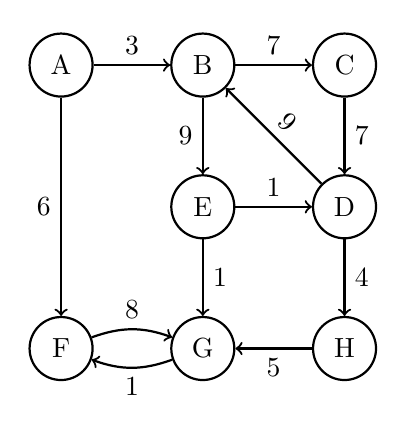
\begin{tikzpicture}[style=thick,scale=0.9]
\tikzstyle{vertex}=[draw, circle, fill=white, inner sep=0pt, minimum size=8mm]

\node[vertex] (A) at (-2, 2) {A};
\node[vertex] (B) at ( 0, 2) {B};
\node[vertex] (C) at ( 2, 2) {C};
\node[vertex] (D) at ( 2, 0) {D};
\node[vertex] (E) at ( 0, 0) {E};
\node[vertex] (F) at (-2,-2) {F};
\node[vertex] (G) at ( 0,-2) {G};
\node[vertex] (H) at ( 2,-2) {H};

\draw[->] (A) -- (B)
    node [above, midway] {$3$};
\draw[->] (A) -- (F)
    node [left, midway] {$6$};
\draw[->] (B) -- (C)
    node [above, midway] {$7$};
\draw[->] (B) -- (E)
    node [left, midway] {$9$};
\draw[->] (C) -- (D)
    node [right, midway] {$7$};
\draw[->] (D) -- (B)
    node [above, midway, sloped] {$9$};
\draw[->] (D) -- (H)
    node [right, midway] {$4$};
\draw[->] (E) -- (D)
    node [above, midway] {$1$};
\draw[->] (E) -- (G)
    node [right, midway] {$1$};
\draw[->] (F) to[bend left=20] node [above, midway] {$8$} (G);
\draw[->] (G) to[bend left=20] node [below, midway] {$1$} (F);
\draw[->] (H) -- (G)
    node [below, midway] {$5$};
\end{tikzpicture}
\caption{Graf za nalogo~\ref{nal:dijkstra}.}
\label{fig:dijkstra}
\end{figure}
\end{vprasanje}
\begin{odgovor}
\end{odgovor}
\end{naloga}

\begin{naloga}{?}{Vaje OR 4.5.2016}
\begin{vprasanje}
Naj bo $G = (V, E)$ graf,
za katerega so dolžine povezav določene s funkcijo $\ell : E \to \R$
(tj., dolžine so lahko tudi negativne).
Definirajmo še funkcijo $\ell' : E \to \R$ tako,
da velja $\ell'(e) = \ell(e) - \min\set{\ell(f)}{f \in E}$
(dolžine, določene z $\ell'$, so torej nenegativne).
Dokaži ali ovrzi: drevo najkrajših poti,
ki ga Dijkstrov algoritem ustvari ob vhodu $(G, \ell')$,
je tudi drevo najkrajših poti za graf $G$ z dolžinami povezav,
določenimi z $\ell$.

\end{vprasanje}
\begin{odgovor}
\end{odgovor}
\end{naloga}


\begin{naloga}%
{Dasgupta, Papadimitriou, Vazirani}{\cite[Exercise~4.13]{dpv}}
\begin{vprasanje}
Denimo, da imamo neusmerjen graf $G = (V, E)$,
katerega vozlišča pred\-stav\-lja\-jo mesta,
povezave pa predstavljajo ceste, ki jih povezujejo.
Za vsako povezavo $e \in E$ poznamo njeno dolžino $\ell_e$ (v kilometrih).

Priti želimo iz mesta $s$ v mesto $t$.
V vsakem mestu je bencinska črpalka, ob cestah pa teh ni.
Žal imamo na voljo samo star avto,
ki lahko s polnim rezervoarjem prepelje le $L$ kilometrov.
\begin{enumerate}[(a)]
\item Zapiši algoritem, ki v linearnem času poišče pot,
ki jo lahko prevozimo z našim avtom,
oziroma ugotovi, da ta ne obstaja.
\item Izkaže se, da z našim avtom te poti ne moremo prevoziti,
zato se odločimo za nakup novega.
Zapiši algoritem, ki v času $O(m \log n)$
določi najmanjše število prevoženih kilometrov,
ki naj jih avto zmore z enim polnjenjem,
da bo pot od $s$ do $t$ mogoča.
\end{enumerate}

\end{vprasanje}
\begin{odgovor}
\end{odgovor}
\end{naloga}


\begin{naloga}{Sergio Cabello}{Vaje OR 7.12.2016}
\begin{vprasanje}
Zasnuj različico Dijkstrovega algoritma
za iskanje najkrajše poti med vozliščema $s$ in $t$ v grafu $G$,
ki iskanje hkrati začne v vozliščih $s$ in $t$.
Kdaj naj se iskanje konča in kako naj se poišče rešitev?
\end{vprasanje}
\begin{odgovor}
\end{odgovor}
\end{naloga}


\begin{naloga}%
{Dasgupta, Papadimitriou, Vazirani}{\cite[Exercise~3.1]{dpv}}
\begin{vprasanje}[nal:dfs]
Na grafu s slike~\ref{fig:bdfs} izvedi iskanje v globino.
V primerih, ko imaš več ena\-ko\-vred\-nih izbir,
upoštevaj abecedni vrstni red.
Za vsako povezavo določi, ali se nahaja v drevesu iskanja v globino.
\end{vprasanje}
\begin{odgovor}
\end{odgovor}
\end{naloga}


\begin{naloga}{Janoš Vidali}{Vaje OR 21.5.2018}
\begin{vprasanje}[nal:bf]
S pomočjo Bellman-Fordovega algoritma
določi razdalje od vozlišča $A$ do ostalih vozlišč
v grafu s slike~\ref{fig:bf}.

\begin{figure}[t]
\centering
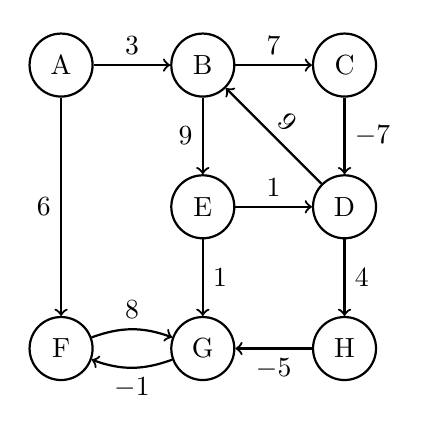
\begin{tikzpicture}[style=thick,scale=0.9]
\tikzstyle{vertex}=[draw, circle, fill=white, inner sep=0pt, minimum size=8mm]

\node[vertex] (A) at (-2, 2) {A};
\node[vertex] (B) at ( 0, 2) {B};
\node[vertex] (C) at ( 2, 2) {C};
\node[vertex] (D) at ( 2, 0) {D};
\node[vertex] (E) at ( 0, 0) {E};
\node[vertex] (F) at (-2,-2) {F};
\node[vertex] (G) at ( 0,-2) {G};
\node[vertex] (H) at ( 2,-2) {H};

\draw[->] (A) -- (B)
    node [above, midway] {$3$};
\draw[->] (A) -- (F)
    node [left, midway] {$6$};
\draw[->] (B) -- (C)
    node [above, midway] {$7$};
\draw[->] (B) -- (E)
    node [left, midway] {$9$};
\draw[->] (C) -- (D)
    node [right, midway] {$-7$};
\draw[->] (D) -- (B)
    node [above, midway, sloped] {$9$};
\draw[->] (D) -- (H)
    node [right, midway] {$4$};
\draw[->] (E) -- (D)
    node [above, midway] {$1$};
\draw[->] (E) -- (G)
    node [right, midway] {$1$};
\draw[->] (F) to[bend left=20] node [above, midway] {$8$} (G);
\draw[->] (G) to[bend left=20] node [below, midway] {$-1$} (F);
\draw[->] (H) -- (G)
    node [below, midway] {$-5$};
\end{tikzpicture}
\caption{Graf za nalogo~\ref{nal:bf}.}
\label{fig:bf}
\end{figure}
\end{vprasanje}
\begin{odgovor}
\end{odgovor}
\end{naloga}


\begin{naloga}{Janoš Vidali}{Vaje OR 7.12.2016}
\begin{vprasanje}[nal:topo]
Dan je usmerjen acikličen graf s slike~\ref{fig:topo}.

\begin{enumerate}[(a)]
\item Poišči topološko ureditev vozlišč zgornjega grafa.

\item Poišči najkrajšo pot od vozlišča $G$ do vozlišča $E$.

\item Poišči najdaljšo pot od vozlišča $G$ do vozlišča $E$.
\end{enumerate}

\begin{figure}
\centering
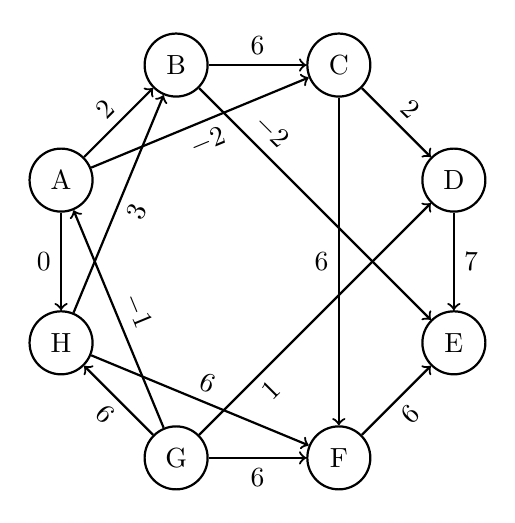
\begin{tikzpicture}[style=thick,scale=0.9]
\tikzstyle{vertex}=[draw, circle, fill=white, inner sep=0pt, minimum size=8mm]

\node[vertex] (A) at (xyz polar cs:angle=157.5,radius=3) {A};
\node[vertex] (B) at (xyz polar cs:angle=112.5,radius=3) {B};
\node[vertex] (C) at (xyz polar cs:angle= 67.5,radius=3) {C};
\node[vertex] (D) at (xyz polar cs:angle= 22.5,radius=3) {D};
\node[vertex] (E) at (xyz polar cs:angle=337.5,radius=3) {E};
\node[vertex] (F) at (xyz polar cs:angle=292.5,radius=3) {F};
\node[vertex] (G) at (xyz polar cs:angle=247.5,radius=3) {G};
\node[vertex] (H) at (xyz polar cs:angle=202.5,radius=3) {H};

\draw[->] (A) -- (B) node [above, midway, sloped] {$2$};
\draw[->] (A) -- (C) node [below, midway, sloped] {$-2$};
\draw[->] (A) -- (H) node [left, midway] {$0$};
\draw[->] (B) -- (C) node [above, midway] {$6$};
\draw[->] (B) -- (E) node [above, near start, sloped] {$-2$};
\draw[->] (C) -- (D) node [above, midway, sloped] {$2$};
\draw[->] (C) -- (F) node [left, midway] {$6$};
\draw[->] (D) -- (E) node [right, midway] {$7$};
\draw[->] (F) -- (E) node [below, midway, sloped] {$6$};
\draw[->] (G) -- (A) node [above, midway, sloped] {$-1$};
\draw[->] (G) -- (D) node [below, near start, sloped] {$1$};
\draw[->] (G) -- (F) node [below, midway] {$6$};
\draw[->] (G) -- (H) node [below, midway, sloped] {$6$};
\draw[->] (H) -- (B) node [below, midway, sloped] {$3$};
\draw[->] (H) -- (F) node [above, midway, sloped] {$6$};
\end{tikzpicture}
\caption{Graf za nalogo~\ref{nal:topo}.}
\label{fig:topo}
\end{figure}
\end{vprasanje}
\begin{odgovor}
\end{odgovor}
\end{naloga}


\begin{naloga}{?}{Kolokvij OR 5.9.2013}
\begin{vprasanje}[nal:oviratlon]
Oviratlon je tekalna preizkušnja
na 8 do 10 kilometrov dolgi poti z različnimi ovirami.
Zanima nas, na koliko različnih načinov lahko pridemo od štarta do cilja.
Dan je utežen usmerjen acikličen graf $G$ ter vozlišči $s$ in $t$,
ki predstavljata štart oziroma cilj.
Uteži na povezavah nam predstavljajo,
na koliko načinov jih lahko prečkamo.

\begin{enumerate}[(a)]
\item Reši nalogo za graf s slike~\ref{fig:oviratlon}.

\item Zapiši algoritem, ki reši dani problem.
Kakšna je njegova časovna zahtevnost?
\end{enumerate}

\begin{figure}
\centering
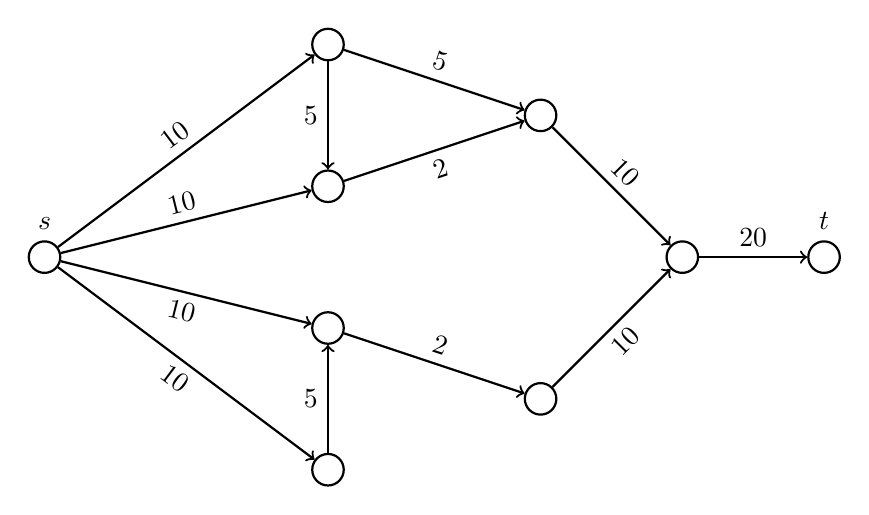
\begin{tikzpicture}[style=thick,scale=0.9]
\tikzstyle{vertex}=[draw, circle, fill=white, inner sep=0pt, minimum size=4mm]

\node[vertex] (S) at (-5, 0) [label=above:$s$] {};
\node[vertex] (A) at (-1, 3) {};
\node[vertex] (B) at (-1, 1) {};
\node[vertex] (C) at (-1,-1) {};
\node[vertex] (D) at (-1,-3) {};
\node[vertex] (E) at ( 2, 2) {};
\node[vertex] (F) at ( 2,-2) {};
\node[vertex] (G) at ( 4, 0) {};
\node[vertex] (T) at ( 6, 0) [label=above:$t$] {};

\draw[->] (S) -- (A)
    node [above, midway, sloped] {$10$};
\draw[->] (S) -- (B)
    node [above, midway, sloped] {$10$};
\draw[->] (S) -- (C)
    node [below, midway, sloped] {$10$};
\draw[->] (S) -- (D)
    node [below, midway, sloped] {$10$};
\draw[->] (A) -- (B)
    node [left, midway] {$5$};
\draw[->] (A) -- (E)
    node [above, midway, sloped] {$5$};
\draw[->] (B) -- (E)
    node [below, midway, sloped] {$2$};
\draw[->] (C) -- (F)
    node [above, midway, sloped] {$2$};
\draw[->] (D) -- (C)
    node [left, midway] {$5$};
\draw[->] (E) -- (G)
    node [above, midway, sloped] {$10$};
\draw[->] (F) -- (G)
    node [below, midway, sloped] {$10$};
\draw[->] (G) -- (T)
    node [above, midway] {$20$};

\end{tikzpicture}
\caption{Graf za nalogo~\ref{nal:oviratlon}.}
\label{fig:oviratlon}
\end{figure}
\end{vprasanje}
\begin{odgovor}
\end{odgovor}
\end{naloga}
